\documentclass[a4paper]{memoir}

\setlength{\trimtop}{0pt}
\setlength{\trimedge}{\stockwidth}
\addtolength{\trimedge}{-\paperwidth}
\settypeblocksize{24cm}{14cm}{*}
\setulmargins{3cm}{*}{*}
\setlrmargins{3.5cm}{*}{*}
\setmarginnotes{17pt}{51pt}{\onelineskip}
\setheadfoot{\onelineskip}{2\onelineskip}
\setheaderspaces{*}{2\onelineskip}{*}
\checkandfixthelayout

\clubpenalty = 10000 
\widowpenalty = 10000 
\displaywidowpenalty = 10000

\usepackage{selinput}
\usepackage{microtype}
\usepackage{graphicx}
\usepackage{hyperref} % muss letztes package sein

\hypersetup{pdfborder=0 0 0}

\title{Designing a Real KERNAL Cartridge}
\author{
Thomas 'skoe' Giesel
(skoe@directbox.com)
}

\begin{document}
\emergencystretch=0.15\hsize

%%%%%%%%%%%%%%%%%%%%%%%%%%%%%%%%%%%%%%%%%%%%%%%%%%%%%%%%%%%%%%%%%%%%%%%%
\pagestyle{empty}
\begin{center}

\vspace*{5cm}
\textsc{\huge Designing a Real KERNAL Cartridge}\\[2cm]
{\large Thomas 'skoe' Giesel}

\vfill

% Bottom of the page
{\large First Edition \\[0.5cm] \today}

\end{center}
%%%%%%%%%%%%%%%%%%%%%%%%%%%%%%%%%%%%%%%%%%%%%%%%%%%%%%%%%%%%%%%%%%%%%%%%

\clearpage

\tableofcontents

\chapter{Introduction}

\section{The Need for a KERNAL Cartridge}

Nearly all Commodore computers contain a KERNAL ROM. The KERNAL ROM
contains the operating system of the machine, providing the drivers
necessary for low level input/output access, among other functions.
However, since the KERNAL is a ROM and cannot be easily modified, it
can be hard to upgrade the functionality in the KERNAL.

On the Commodore 64, the KERNAL is used to access the serial bus and
therefore the disk drives. Most often, people look to KERNAL
upgrades to address slow disk access issues.  The standard KERNAL
drivers in the C64 offer only slow transfer functionality, while
there are many replacement KERNAL offerings that allow greatly
enhanced transfer functionality.  However, this is not the only
reason a KERNAL replacement might be desired.  Auto-boot
functionality, customized screen layout, or other reasons might
demand a KERNAL replacement.

While there are alternative ways to
replace some KERNAL functionality, those mechanisms limit
usefulness.  Changing KERNAL vectors that are located in RAM only
applies to callers that utilize those vectors, and only vectorized
functionality can be enhanced.  As well, new functionality must
exist in the address space, which might conflict with application
code.  Thus, cartridges like Action Replay, Fastload, or The Final
Cartridge III cannot always offer the level of compatibility
desired.

One well-known replacement KERNAL is JiffyDOS. To use JiffyDOS, one
must replace the KERNAL ROM in the host machine with a new ROM,
while the operating system of each drive must be upgraded as well.
Though, some drives, like CMD devices and sd2iec-based devices,
support JiffyDOS standard.

Disk drives typically socket their DOS ROM, for easy replacements.
However, many computer systems do not socket the KERNAL ROM, making
replacement much harder.

A KERNAL cartridge can address these issues.  The cartridge would
allow the same functionality as a KERNAL replacement, but would not
require disassembly of the computer system or soldering of a socket
to the circuit board to allow replacement.

\section{KERNAL Cartridge Design Challenges}

When not in "Ultimax" mode, which radically changes the memory map
to mimic the layout in the Commodore Ultimax system, The KERNAL can
be found in the C64 address space at \$E000 to \$FFFF, an 8KiB
section of memory. But the KERNAL is not the only memory in this
address space. There is also RAM below the KERNAL. Programs can
decide if they want to read the KERNAL ROM or the RAM there by
setting the HIRAM bit in the I/O register \$01 of the 6510 CPU.
Figure \ref{fig:memory-map-plain} shows the memory map of the C64
with no cartridge attached.

\begin{figure}
    \centering
    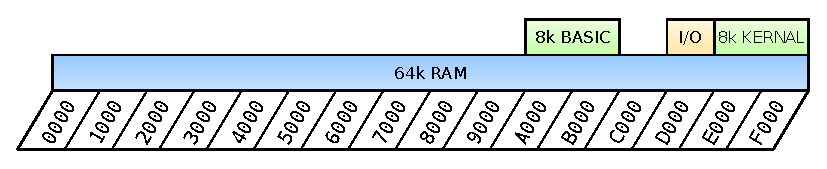
\includegraphics[width=15cm]{src/memory-map-plain}
    \caption{Memory map of the C64 with no cartridge attached}
    \label{fig:memory-map-plain}
\end{figure}

Write accesses from the CPU are always done to the RAM below the
KERNAL. The VIC-II always reads from that RAM but not from the KERNAL
ROM. But CPU read accesses depend from the signal \#HIRAM, which is
set in bit 1 of the I/O register \$01. If \#HIRAM is low (0), RAM
is read. If it is high (1), KERNAL ROM is read. Figure \ref
{fig:memory-map-hiram} shows this mechanism.

\begin{figure}
    \centering
    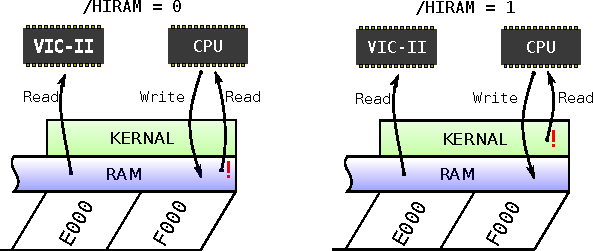
\includegraphics[width=11cm]{src/memory-map-hiram}
    \caption{HIRAM controls access to KERNAL memory space}
    \label{fig:memory-map-hiram}
\end{figure}

A compatible KERNAL cartridge must implement this behavior.
Otherwise, programs which use \$01 to hide the KERNAL ROM will fail,
because they cannot use the RAM between \$E000 and \$FFFF. However,
the \#HIRAM signal is not available on the Expansion Port. That is why
many KERNAL cartridges either do not provide access to this RAM area
or have to use a wire which must be connected to the \#HIRAM signal
inside the C64.

For a compatible KERNAL cartridge with no additional wire, the
cartridge must use another method to determine the state of /HIRAM.
Since a write to address \$01 sets the state of /HIRAM, one obvious
idea involves tracking any writes to \$01. However, writes to \$00
and \$01 do not present data on the C64 data bus, rendering such a
solution ineffective.

\chapter{KERNAL Cartridge Design}

\section{Working principle}

\#HIRAM does not act alone in re-arranging the memory map. Two lines
on the expansion port, \#GAME and \#EXROM, also play a part in
configuring the memory map.

Pulled up via resistors inside the C64, the two lines can be
configured via an external cartridge. When there is no cartridge
attached both of them are high (1). When a cartridge is attached it
can pull one or both of these lines low (0) to change the memory
configuration. When a cartridge is attached, the memory
configuration can still be configured with the 6510 I/O port, e.g.,
to hide the cartridge ROM.

There are two more control lines on the Expansion Port: \#ROML and
\#ROMH. Excepting Ultimax mode, \#ROML selects an external
cartridge ROM into \$8000-\$9FFF, while \#ROMH selects a ROM into
\$A000-\$BFFF. Whenever the C64, via the address mapping logic in
the Programmable Logic Array (PLA), decides that data from a
cartridge must be read, it pulls down one of these lines.
Traditionally they are connected directly to two 8 KiB ROM ICs in
the cartridge.

An example: A cartridge pulls down \#GAME and \#EXROM to tell the C64
that there is a 16 KiB cartridge attached. The currently running
program has not disabled ROM by leaving \#HIRAM and \#LORAM as 1. When
the program wants to read a byte at \$A123, which is in the upper
cartridge ROM, the PLA determines that this byte must be read from
the external cartridge and brings \#ROMH active (0).

Table \ref {tab:game-exrom} shows the configurations which can be
set by a cartridge using \#GAME and \#EXROM.

\begin{table}
    \centering
    \begin{tabularx}{\textwidth}{ccX}
        \toprule
        GAME & EXROM & Memory Map \\
        \midrule
        1 & 1 & No cartridge attached, memory map unchanged \\[3pt]
        1 & 0 & 8 KiB cartridge, \#ROML mapped to \$8000..\$9FFF \\[3pt]
        0 & 0 & 16 KiB cartridge, \#ROML mapped to \$8000..\$9FFF, \#ROMH mapped to \$A000..\$BFFF \\[3pt]
        0 & 1 & Compatibility mode to Commodore MAX, Ultimax mode,
                \#ROML mapped to \$8000..\$9FFF, \#ROMH mapped to \$E000..\$FFFF \\[3pt]
        \bottomrule
    \end{tabularx}
    \caption{Configurations of \#GAME and \#EXROM}
    \label{tab:game-exrom}
\end{table}

In \cite[Ch.~3]{HS10} xxxxxxxxx several different 
memory configurations are described. Some interesting cases are
shown in table \ref {tab:mem-configs}. In columns (1), (2) and (3) no cartridge is
attached, i.e. \#GAME and \#EXROM are 1. Only \#HIRAM controls
whether there is RAM or KERNAL ROM visible to the CPU at \$E000 in
this these cases.

\begin{table}
    \centering
    \begin{tabularx}{\textwidth}{lccccccc}

        \toprule
        \#LORAM & 1 & x & 0 & x & 0 & 1 & x \\[3pt]
        \#HIRAM & 1 & 0 & 1 & 1 & 0 & 0 & x \\[3pt]
        \#GAME  & 1 & 1 & 1 & 0 & 0 & 0 & 0 \\[3pt]
        \#EXROM & 1 & 1 & 1 & 0 & 0 & 0 & 1 \\[3pt]
        \midrule
        E000-FFFF & \textbf{Kernal} & \textbf{RAM} & \textbf{Kernal} &
          Kernal         & Kernal        & RAM           & \textbf{ROMH} \\[3pt]
        A000-BFFF & BASIC            & RAM           & RAM              &
          \textbf{ROMH} & \textbf{RAM} & \textbf{RAM} & --- \\[3pt]
        \bottomrule
    \end{tabularx}
    \caption{Memory configurations}
    \label{tab:mem-configs}
\end{table}

There is also a memory area controlled by HIRAM which results in a
control signal visible at the Expansion Port: When a 16 KiB
cartridge is attached to the Expansion Port, /HIRAM is used to
select whether the \#ROMH part of the cartridge or the internal RAM
is mapped to \$A000. This is shown in columns (4), (5) and (6).

This proves invaluable for external KERNAL cartridge design. If the
cartridge sets the \#GAME and \#EXROM lines low, and a read
access of \$A000-\$BFFF occurs, \#ROMH provides the state of
\#HIRAM. As \#ROMH is connected to the Expansion Port, it can be
captured by the cartridge.

However, the cartridge needs to know the state of \#HIRAM during 
accesses to \$E000-\$FFFF, not \$A000-\$BFFF. The KERNAL
cartridge must force an access to \$A000-\$BFFF, but it cannot
change any running application code. Given those requirements, the
cartridge must find a way to drive the address bus itself in a way
that does not affect the running application.

When the CPU wants to read something, it sets its address outputs to
the address to be read. This address must be altered by the KERNAL 
cartridge to detect the state of \#HIRAM. But this must be done 
carefully, because it fights against the CPU address
line drivers and could overheat them when being used excessively.

The 6510 CPU has the ability to turn off its address line
drivers, via a control input called Address Enable Control (AEC). If
this input is low, the CPU effectively deactivates the address line
drivers. Unfortunately AEC is not connected to the Expansion
Port directly. But it is driven by the \#DMA signal, which is
available on the Expansion Port. Unfortunately, \#DMA also changes
the state of another CPU control line, Ready (RDY), which will stop
the CPU.

The 6500 CPU family datasheet shows that when RDY is asserted during a Phi2 cycle and released before the cycle ends, 
it should be ignored and should not stop the CPU. 
Thus, it seems like if the cartridge asserts \#DMA during a Phi2 cycle but releases it before the cycle ends, 
it could drive the address bus during that cycle.
With access to the address bus, the cartridge could drive the address bus to a location within \$A000-\$BFFF
during the cycle, and capture the state of \#HIRAM on the \#ROMH Expansion Port line.

The mechanism was tested on different C64 models. 
It turned out that some machines got unstable and crashed occasionally.
Obviously, the use of the RDY line as described above renders the CPU unstable.

As a next step a method was tried which does not involve \#DMA.
Whenever a CPU read access to the address range \$F000-\$FFFF is detected, 
the cartridge pulls down the address line A13 for a fraction of the clock cycle.
This changes any address between \$F000-\$FFFF to an address between \$A000-\$BFFF.
After this is done, the state of \#HIRAM can be read from \#ROMH.

With these findings we can lay out the steps for cartridge operation:

\begin{itemize}
\item Set /GAME and /EXROM high (memory map: no cartridge attached)
\item Wait until Phi2 is high (CPU cycle) and address bus is stable
\item If it is a read access and the address is in KERNAL space $E000..$FFFF:
    \begin{itemize}
    \item Pull down A13 to alter the address bus to an address in the range 0xA000..0xBFFF
    \item set /GAME and /EXROM to 0 to act like a 16 KiB cartridge, wait
    \item Look at /ROMH to see whether ROM or RAM is selected by HIRAM
    \item \textit{How to send the right byte to the CPU?}
    \end{itemize}
\end{itemize}

If the CPU accesses the KERNAL ROM, the cartridge must place the external KERNAL ROM into the address space at \$E000-\$FFFF.
The memory map shows a way to accomplish that.
Configuration (7) in table \ref {tab:mem-configs} illustrates "Ultimax" mode.
In this mode, any read access in the range \$E000-\$FFFF will activate the \#ROMH signal and will read from external memory.
Therefore, if a valid KERNAL read access is requested, the cartridge must set \#GAME to active (0) and release \#EXROM.
If RAM is to be read instead, the cartridge releases all lines to allow an ordinary RAM access.
When the Phi2 cycle ends, the cartridge releases all lines in any case to return to idle state.

\begin{itemize}
\item Set /GAME and /EXROM high (memory map: no cartridge attached)
\item Wait until Phi2 is high (CPU cycle) and address bus is stable
\item If it is a read access and the address is in KERNAL space $E000..$FFFF:
    \begin{itemize}
    \item Pull down A13 to alter the address bus to an address in the range 0xA000..0xBFFF
    \item Set /GAME and /EXROM to 0 to act like a 16 KiB cartridge, wait
    \item Look at /ROMH to see whether ROM or RAM is selected by HIRAM
    \item Release /EXROM to go to Ultimax mode
    \item When /ROMH is asserted, put the data byte from KERNAL ROM on the bus
    \item Release all lines after Phi2 cycle has ended
    \end{itemize}
\end{itemize}

\section{Timing Considerations}

Some of the steps needed for the external Kernal implementation have
to consider timing requirements of the components of the C64. Most
of them can be found in data-sheets.

\begin{itemize}
\item Wait until Phi2 is high (CPU cycle) and address bus is stable
\end{itemize}

When Phi2 goes high the VIC sets AEC high when it wants to allow a
CPU cycle. After this signal reached the CPU, it takes up to $T_{AES} =
75 ns$ according to the 6510 data-sheet until the address bus shows
the final value. However, measurements done on different types of
C64s have shown that the time between the rising edge of Phi2 and a
stable address bus is significantly smaller. Examples are shown in
figure \ref {fig:addr250407} and figure \ref {fig:addr250469}.

\begin{figure}
    \centering
    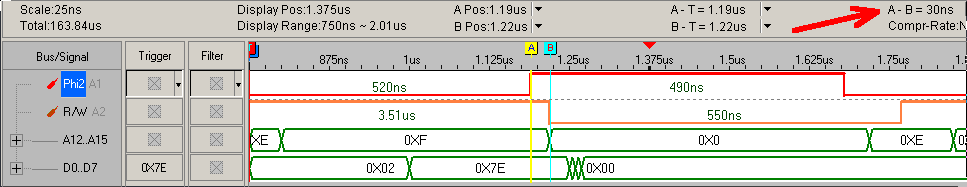
\includegraphics[width=1.1\textwidth]{src/phi2-data-bus-250407}
    \caption{Address Bus after H-Edge of Phi2, Board 250407}
    \label{fig:addr250407}
\end{figure}

\begin{figure}
    \centering
    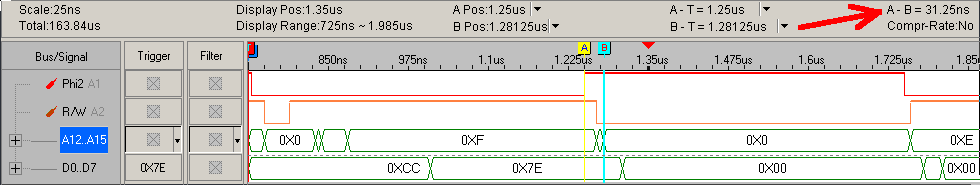
\includegraphics[width=1.1\textwidth]{src/phi2-data-bus-250469}
    \caption{Address Bus after H-Edge of Phi2, Board 250469}
    \label{fig:addr250469}
\end{figure}

To be on the safe side the external Kernal Cartridge will sample the
address bus at $t \ge 80 ns$, where $t = 0$ is the rising edge of Phi2.

\begin{itemize}
\item Assert the /DMA line, wait
\end{itemize}

When the Kernal cartridge pulls down /DMA at $t >= 80 ns$, the CPU
will tristate its address output. The 6510 datasheet states that
this takes up to $T_{AED} = 120 ns$. Interestingly the VIC-II takes over
the address bus already about 50 ns after it disabled AEC. The external
KERNAL implementation modifies the address bus after 80 ns.

\begin{itemize}
\item Look at /ROMH to see whether ROM or RAM is selected by HIRAM
\end{itemize}

The data-sheet of the Signetics 82S100 PLA specifies a typical
propagation delay TPD of 35 ns and a maximum delay of 80 ns. The
Sharp custom IC used in newer C64s has different timings for
different output lines, but in the same ballpark.

We will read the result 80 ns after having set all
input conditions. This is also the time when we release \#DMA to
allow the CPU to restore the address bus. Less than $T_{AES} = 75 ns$
later the address lines are stable again, the flash or RAM memory
chip can select the right data byte. As soon as the PLA pulls down
\#ROMH again. \#OE of the right memory chip is pulled down and the
cartridge can put the data byte onto the bus. When a 55 ns flash is
used, these delays will be together less than about 130 ns. The
remaining time is the Data Stability Time Period ($T_{DSU} \ge 100 ns$)
for the 6510 data lines. All times to measured by the cartridge can
be implemeted as multiple of 40 ns. Therefore a CPLD with a 25 MHz
clock may be used to build the cartridge. As the C64 signals come
from another clock domain, the accuracy is also only 40 ns. Fig
\ref {fig:timing} shows the expected timing.

\begin{figure}
    \centering
    \includegraphics[width=10cm]{src/implemented-timing}
    \caption{Timing of the External KERNAL Cartridge}
    \label{fig:timing}
\end{figure}

\chapter{Implementation}

\section{EasyFlash 3}

The multi-function cartridge EasyFlash 3 contains, among other 
cartridge modes, a KERNAL implementation based on this document. The
cartridge contains flash memory, SRAM, a 25~MHz clock source and a
144 macrocell CPLD.

The hardware design files are released under the Creative Commons
license CC~BY-SA~3.0. They are available at the public repository
\url{https://bitbucket.org/skoe/easyflash/src/tip/Hardware/ef3-kicad/}.

The CPLD core implemented in VHDL is licensed under the zlib
license. It is also available in that repository:
\url{https://bitbucket.org/skoe/easyflash/src/tip/Hardware/ef3-vhdl}.
The file \texttt{architecture.txt} in the repository contains a
detailed description of the implementation.

\cite[Ch.~3]{HS10}

\begin{thebibliography}{999}
\bibitem [HS10]{HS10} Charles Hawkins, Jaume Segura. Introduction to Modern
Digital Electronics. Scitech Pub Inc, Preliminary, 2010
\end{thebibliography}


Commodore 64 Programmer's Reference Guide
Commodore Computers (Author)
Publisher: Financial Times Prentice Hall (April 1983)
ISBN-10: 0672220563
ISBN-13: 978-0672220562
 Product Dimensions:  21.6 x 15.5 x 3.3 cm


\end{document}

